
\begin{center}
    \Huge{\textbf{\underline{Exercise 1}}}
\end{center}

\vspace{0.5cm}

Let \( L \in \{0,1\}^{*} \) be a language formed by the entities X, Y, and Z:
\begin{itemize}
    \item \textbf{X} : Starts with '0' and contains no consecutive '0's.
    \item \textbf{Y} : Starts with '1', followed by a sequence with an even number of '0's.
    \item \textbf{Z} : Starts with either two '0's or two '1's, followed by a sequence of '0's and '1's, and does not contain '101'.
\end{itemize}

Construct the corresponding automaton to recognize all these entities.
\vspace{1cm}
\begin{prettyBox}{Note}{red}
Never loop on the start state, as this can lead to undesired behavior. Doing so makes having independent branches impossible since the
compiler has only one automaton to match all entities.
\end{prettyBox}

\vspace{1.5cm}

\textbf{\underline{\Large{Solution}} :}

\begin{center}
    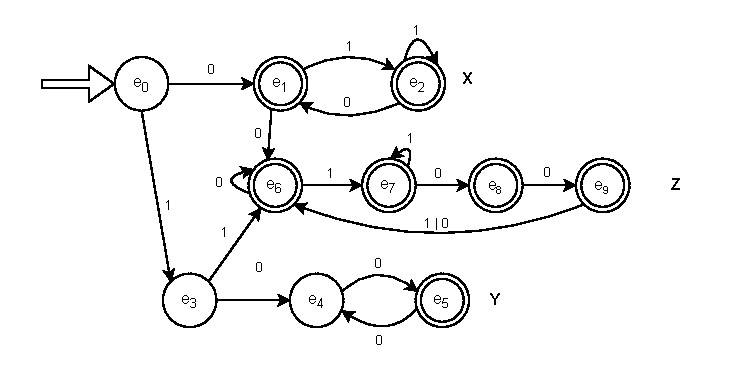
\includegraphics[width=0.8\textwidth]{Exercices/EX1/ex1.drawio.pdf}
\end{center}


